\chapter{Research Methodology}
\label{Chapter2} % For referencing this chapter elsewhere, use \ref{Chapter3}

\section{Research design} \label{design}
For the proposed research, a rigorous framework has been formalized by \parencite{morris_using_2019} and will be referred to as (ADMEP). As \parencite{morris_using_2019} states, "Simulation studies are used to obtain empirical results about the behavior of statistical methods in certain scenarios, as opposed to analytic results", which is at the foundation of the objectives of this research. In essence, this study aims to produce results that "accurately" represent the efficacy of the Random Survival Forest \parencite{ishwaran_random_2008} and the Cox proportional hazards model \parencite{cox_regression_1972}. 

\begin{figure}[h]
 \centering
 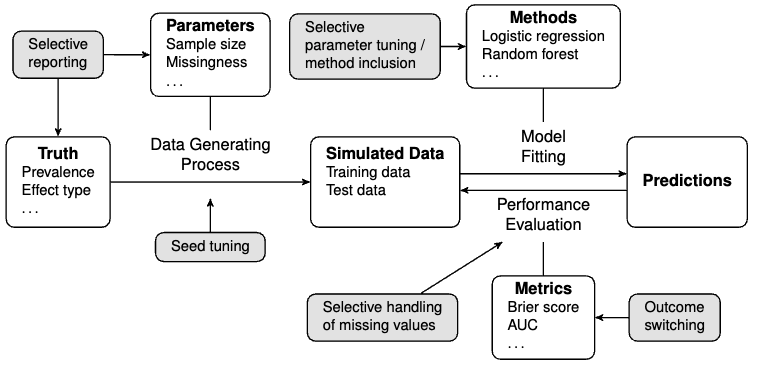
\includegraphics[scale=0.48]{Figures/METHOD_GRAPH.png}
 \caption{\parencite{pawel_pitfalls_2024} Shows a common example of a simulation study plan.}
\end{figure}

\noindent Taking inspiration from the the application of ADMEP by \parencite{pawel_pitfalls_2024}, the following sections define the research broadly:

\subsection{Aims}
\begin{itemize} 
\item To evaluate how effectively the Random Survival Forest and Lasso-Cox models predict survival outcomes.
\item To understand model behavior under varying conditions of data complexity and censoring rates.
\item Document research practices when conducting this study.
\end{itemize}

\subsection{Data-generating mechanisms}
\begin{itemize}
\item Simulate datasets with packages like \parencite{davidson-pilon_lifelines_2024} to introduce complexities like varying censoring rates and non-linear effects.
\item Introduce multicollinearity and various interaction effects to challenge the models' assumptions and robustness.
\end{itemize}

\subsubsection{Missing Data Imputation}

As discussed in \ref{impute} we look at the methods for producing missing value imputation under the CAR and CNAR assumptions.
\\\\
\textit{Delta-adjusted Method} \parencite{jin_imputation_2024}
\begin{equation} \label{eq:deltaadjust}\lambda_{post}(t|Z_{i},X_{i}(t)) = \lambda_{\emptyset}(t|Z_{i},X_{i}(t)) = \lambda_{0}(t)\exp^{(1-\emptyset)\beta Z_{i} + \alpha X_{i}(t)}, t>C_{i}\end{equation}
\noindent The sensitivity parameter (\(\emptyset\)) represents a discounted proportion of the log-hazard ration \(\beta\) under the CNAR assumption. The method assumes that the hazard of having an event for censored subjects is multiplicatively decreased by a factor depending on the \(\emptyset\). The term \((1- \emptyset)\beta\) suggests a reduced effect of the treatment on the hazard rate post-censoring.
\\\\
\textit{Tipping point Analysis} \parencite{jin_imputation_2024}
\par \noindent This method is used to identify how much the assumption of noninformative censoring (CAR) would need to be violated for the study results to become statistically nonsignificant. It uses the delta-adjusted method's parameter \(\emptyset\) to calculate the minimum shift in \(\beta\) (log HR) needed to nullify the treatment effect.
\\\\
\textit{Jump to Reference} \parencite{jin_imputation_2024}
\begin{equation} \label{eq:jtor}\lambda_{post}(t|Z_{i},X_{i}(t)) = \lambda_{J2R}(t|Z_{i},X_{i}(t)) = \lambda_{ref}(t|X_{i}(t)) = \lambda_{0}(t)\exp^{\alpha X_{i}(t)}, t>C_{i}\end{equation}
\noindent This Method assumes that once censored, the hazard rate for a subject from the treatment group immediately aligns with that of the reference group, completely disregarding any residual effects of the treatment past the point of censoring.
\\\\
\textit{Copy Reference} \parencite{jin_imputation_2024}
\begin{equation} \label{eq:copyref}\lambda_{CR}(t|Z_{i} = 1,X_{i}(t)) = \lambda(t|Z_{i} = 0, X_{i}(t)) = \lambda_{0}(t)\exp^{\alpha X_{i}(t)} \text{for all}, t\end{equation}
\noindent This method is conservative but less so than J2R in that it assumes that if a subject in the treatment group is censored, their hazard function matches that of the reference group for the remainder of the study. It does not account for any time-specific variations in hazard that might have been influenced by the treatment before censoring.
\\\\
\textit{Censored at Random (CAR)} \parencite{jin_imputation_2024}
\par \noindent Assumes noninformative censoring where the post-censoring hazard (\(\lambda_{post}\)) is identical to the pre-censoring hazard, simplifying the imputation process.

Hazard post CAR: 
\begin{equation} \label{eq:carassmp}\lambda_{post}(t|Z_{i},X_{i}(t)) = \lambda_{0}(t)\exp^{\beta Z_{i} + \alpha X_{i}(t)}, t>C_{i}\end{equation}

Hazard post CNAR:
\begin{equation} \label{eq:cnarassmp}\lambda_{post}(t|Z_{i},X_{i}(t)) \neq \lambda_{0}(t)\exp^{\beta Z_{i} + \alpha X_{i}(t)}, t>C_{i}\end{equation}

\subsubsection{Data Simulation}
\textit{Parametric Distribution}
\par \noindent This method is used to simulate survival times using predefined parametric distributions. The fit of each distribution to the data is tested using the one-sample Cramér-von Mises (CVM) test \parencite{thurow_how_2023}. The distribution that shows the least deviation from the data (highest p-value in the CVM test) is chosen for simulation. Parameters for these distributions are estimated using Maximum Likelihood Estimation (MLE). An Example of mixed distribution: 
\begin{equation} \label{eq:paramdist}f(x)=0.2.f_{Weibull}(\alpha,\lambda)+0.8.f_{norm}(\mu,\sigma)(x)\end{equation}
\noindent Where \(f_{Weibull(\alpha, \lambda)}\) and \(f_{norm}(\mu,\sigma)\) are the density functions for the Weibull and normal distributions, respectively.
\\\\
\textit{Kernel Density Estimation (KDE)}
\par \noindent Used to estimate by utilizing the density function of the data for simulation. The density function is estimated using the kdensity function from the \parencite{thurow_how_2023} R-package, which employs a Gaussian kernel. The Accept-reject method is used to generate random values that follow the estimated density function. Draw \((X, U)\) from the joint distribution \((X, U) ~ \left\{ (x,u):0<u<f(x)\right\}\) where X is a random variable following the estimated density f, and U is uniformly distributed between 0 and \(f(x)\). If \(u_{i} < f(x_{i})\) for a sampled \((X,U),x_{i}\) is accepted as a realization from the density function \(f\)
\\\\
\textit{Case Resampling}
\par \noindent Simulate data by resampling observed data points with replacement. Directly resample observations (ti, di) from the existing dataset of observed times and censoring indicators. \((t_{i}, d_{i})^{*}\) are drawn with replacement from \(\left\{ (t_{1}, d_{1}) \dots (t_{n}, d_{n})\right\}\)
\\\\
\textit{Conditional Bootstrapping}
\par \noindent To simulate data using bootstrapping that accounts for censoring, this helps sample censor times. For censored observations, censoring times are carried over to the simulated data. For uncensored observations, new censoring times are sampled based on the conditional distribution of censoring times given they are greater than the observed event time. Censoring Time for censored data: \(c_{i}^{*} = t_{i}\) for censored observation. Censoring Time for uncensored data: \(c_{i}^{*}\) is sampled from \(G_{i}(c) = \frac{G(c)-G(t_{i})}{1-G(t_{i})}\) where \(G\) is the distribution function of censoring times and \(t_{i}\) is the observed event time. Event times \(t^{*}_{oi}\) are sampled from the observed event times with replacement. \parencite{thurow_how_2023} Show that the reconstruction of reliable benchmark data sets is meticulously reconstructed from published Kaplan-Meier plots and other vital statistics like hazard ratios and p-values from log-rank tests. The data sets, particularly those with non-crossing survival curves, demonstrate high fidelity to the original data, proving them to be excellent resources for subsequent model evaluations.
\subsubsection{Synthetic Data Generation}
\noindent \parencite{norcliffe_survivalgan_2023} Employ several metrics to assess synthetic survival data according to the real dataset. They help identify and correct biases in synthetic data to better align with real-world data, enhancing the credibility of survival analysis models. The optimism metric assesses whether the synthetic data is over-optimistic or over-pessimistic compared to real data by comparing the expected lifetimes derived from Kaplan-Meier (KM) plots.
\begin{equation} \label{eq:optimisim}\text{Optimism} = \frac{1}{T} \int_{0}^{T}(S_{Syn}(t)-S_{Real}(t))dt\end{equation}
\noindent Where \(S_{Syn}(t) and S_{Real}(t)\) are the synthetic and real Kaplan-Meier survival functions respectively, and T is the latest time point available. The optimism metric ranges between -1 and 1, where values closer to 0 indicate accurate lifetime predictions, positive values suggest over-optimism, and negative values indicate over-pessimism. The short-sightedness metric quantifies how much earlier synthetic data, discontinues providing predictions compared to real data, reflecting potential censorship in the synthetic modeling.
\begin{equation} \label{eq:ssmetric}\text{Short-Sightedness} = \frac{T_{Real}-T_{Syn}}{T_{Real}}\end{equation}
\noindent Here, \(T_{Syn} and T_{Real}\) are the end times of the synthetic and real Kaplan-Meier plots, respectively. This metric ranges from 0 to 1, where 0 indicates no censorship issues and 1 indicates complete short-sightedness in the synthetic data predictions. Lastly, the Kaplan-Meier divergence measures the overall divergence between the synthetic and real KM curves across the observed time, providing a comprehensive measure of similarity between the two datasets.
\begin{equation} \label{eq:kmdiverge}\text{KM Divergence} = \frac{1}{T}\int_{0}^{T}|S_{Syn}(t)-S_{Real}(t)|dt\end{equation}
\noindent This formula calculates the mean absolute difference between the synthetic and real survival functions over time, scaled by the total duration observed. The KM divergence values range from 0 to 1, where 0 indicates perfect matching KM curves and 1 represents the maximum possible difference.

\subsection{Methods}
\begin{itemize}
\item Random Survival Forest: Implement using a combination of proposed packages in \ref{methods}, tuning tree-related parameters.
\item Lasso-Cox Model: Use a combination of the proposed packages in \ref{methods} for implementing Cox regression with Lasso regularization, optimizing the regularization strength and model complexity. 
\item Explore integration effects from the different packages.
\end{itemize}

\subsubsection{Cox Proportional Hazards Model}
The proposition consists of covariates, known as attributes regarding a unit in a distribution of data, which is associated with a coefficient \(\beta\) scaling the impact of said covariates; this product is then bound by the baseline hazard \(h_{0}(t)\).
\begin{equation} \label{eq:cox}h(t|X) = h_0(t) \exp(\beta_1 X_1 + \beta_2 X_2 + \ldots + \beta_n X_n)\end{equation}
An assumption of the Cox model is the proportional hazards assumption, suggesting that the hazard ratios for different covariates remain constant over time we see this for two events observations. This is an operational Assumption and a limitation as this is not always true for survival data. 
\begin{equation} \label{eq:coxph}\frac{h(t|X_1)}{h(t|X_2)} = \frac{h_0(t) \exp(\beta^T X_1)}{h_0(t) \exp(\beta^T X_2)} = \frac{\exp(\beta^T X_1)}{\exp(\beta^T X_2)} = \exp(\beta^T (X_1 - X_2))\end{equation}
The model can handle censoring, by adjusting the likelihood function for observations where event occurrence did not happen in a particular continuous time frame, and by maximizing the likelihood of all observed events, it is possible to estimate the coefficients that could work the best under the Cox formulation.
\begin{equation} \label{eq:coxlikely}L(\beta) = \prod_{i: \delta_i = 1} \frac{\exp(\beta^T X_i)}{\sum_{j \in R(t_i)} \exp(\beta^T X_j)}\end{equation}

\subsubsection{Lasso Regularisation}
\noindent The Lasso technique \parencite{tibshirani_regression_1996}, a regression analysis method introduced to address specific limitations of Ordinary Least Squares (OLS) estimation, is particularly beneficial in scenarios with a large number of predictors or high collinearity among them which would mean that models could produce inflated variance scores, and cause impaired interpretability. Lasso optimizes prediction accuracy and enhances model interpretability by employing a shrinkage process that can set certain coefficients to zero effectively, thus performing variable selection.
\begin{equation} \label{eq:lasso}\hat{\beta}^{lasso} = \arg \min_{\beta} \left\{ \frac{1}{2N} \sum_{i=1}^{N} (y_i - \beta_0 - \sum_{j=1}^{p} X_{ij}\beta_j)^2 \right\}\end{equation}
bound by,
\begin{equation} \label{eq:lassobound}\sum_{j=1}^{p} |\beta_j| \leq t.\end{equation}
\noindent \parencite{freijeirogonzalez_critical_2022} The inclusion of the regularisation term, is crucial as it allows for the reduction of model complexity by penalizing the magnitude of the coefficients, which promotes sparser models. This sparsity is instrumental in enhancing interpretability by isolating only the most significant predictors that contribute to the dependent variable. The objective function of LASSO is convex for \(l_{1}\) norm, which simplifies finding the global minimum. Multiple optimal solutions might exist, especially when the number of predictors \(p\) exceeds the number of observations \(n\). \parencite{freijeirogonzalez_critical_2022} LASSO introduces bias in the coefficients to achieve lower variance and better model parsimony. Consistent under conditions like the irrepresentable condition, crucial for variable selection. Bias Correction achieved via,
\begin{equation} \label{eq:lassobais}\hat{\beta}_{j}^{LASSO}=sign(\hat{\beta}_{j}^{OLS})(|\hat{\beta}_{j}^{OLS}| - \lambda)_{+}\end{equation}

\subsubsection{Random Survival Forest}
\noindent Random survival forests \parencite{ishwaran_random_2008} are an extension of random forests, which can handle right-censored data and aim to estimate the appropriate survival function. Consisting of an ensemble of trees \parencite{ishwaran_random_2008}, which are grown from a bootstrap sample, and each node of underlying trees, consists of specific covariates due to a random selection of features for splits in each tree.
\\\\
\noindent Per node splitting criteria are conditional to survival time and censoring, whereby node “impurity” \parencite{ishwaran_random_2008} is determined by the survival differences. Methods like log-rank, conservation of events splitting rule, and random log-rank are used. Terminal nodes are the result of saturated splitting criteria, with each endpoint having d-dimensional covariates of the individuals encapsulated. 
\\\\
\noindent A key component of the model is the conservation of events principle, which is used to define a type of predicted outcome, namely ensemble mortality, which is derived from the cumulative hazard function (CHF) using the Nelson-Aalen estimator in the original paper by \parencite{ishwaran_random_2008}. 
\\\\
\noindent Terminal nodes or nodes at the end of tree branches all share the estimated hazard function. Another key concept is the out-of-bag (OOB) samples which act as a validation subset \parencite{ishwaran_random_2008}. 
\\\\
\noindent The OOB error is calculated on the ensemble survival function of the observed data using metrics like concordance (C-index). Used for estimating prediction error and model performance without a separate test data set. Each tree's error is calculated using data not included in its training set (out-of-bag). Prediction error metrics, like the concordance index which calculates the permissible pairs per node and OOB prediction error, are used for accuracy metrics. 

\begin{equation} \label{eq:ooberror}
\hat{\Lambda}_{oob}(t,x_{i}) = \frac{1}{\sum_{b=1}^{B}I(x_{i}\in L^{b}_{oob})}\sum_{b=1}^{B}I(x_{i}\in L^{b}_{oob})\hat{\Lambda}_{b}(t,x_{i})
\end{equation}


\subsection{Estimands}
\begin{itemize}
\item Focus on estimations, like survival functions, hazard ratios, etc. for both models and survival probabilities at specified time points.
\item Bootstrap samples to build confidence intervals for key estimands, ensuring the robustness of the findings.
\item Analyze feature importance in RSF and assess how Lasso regularization affects the selection of covariates in the Cox model.
\end{itemize}

\subsubsection{Lasso Penalised Cox Proportional Hazards}
The log partial likelihood for the Cox model, as given by:

\begin{equation} \label{eq:likelihood}l(\beta) = \sum_{i:\delta_{i}=1} \left[ \beta^{T}x_{i} - \log{\sum_{j:t_{j}\ge t_{i}} \exp(\beta^{T}x_{j})} \right]\end{equation}

\noindent Which provides a measure of how well the model's predicted hazards match the observed data. Here, \(\delta\) indicates whether an event (e.g., failure, death) was observed at time \(t_{i}\). 

\subsubsection{Random Survival Forests}
Random forests are adapted for survival analysis by modifying how predictions are aggregated to handle censored data effectively. Forest survival function estimator:
\begin{equation} \label{eq:rsfestimator}\hat{\Lambda}(t, x_{0}) = \frac{1}{B} \sum_{b=1}^{B} \hat{\Lambda}_{b}(t,x_{0})\end{equation}
Survival function:
\begin{equation} \label{eq:survrsf}S(t,x_{0}) = \exp^{-\hat{\Lambda}(t,x_{0})}\end{equation}

\noindent Variable importance (VI) \parencite{pham_springer_2023} in random forests is used to rank variables based on their contribution to prediction accuracy. It is assessed by looking at each predictor variable in the sample and assessing the impact on prediction error, an increase in error indicating importance. Different random forest settings can yield different importance rankings due to the model's sensitivity to the configuration. VI is shown by \parencite{pham_springer_2023}:
\begin{equation} \label{eq:vinorm}
VI(j) = \frac{1}{B}\sum_{b=1}^{B}(\frac{Err(j)_{b}}{Err_{b}}-1)
\end{equation}

\noindent VI Adaptation:
\begin{equation} \label{eq:viadapt}VI(j) = \frac{1}{B}\sum_{b=1}^{B}(\frac{Err(j|Z)_{b}}{Err_{b}}-1)\end{equation}

\noindent This adaptation \ref{eq:viadapt} addresses correlations \parencite{pham_springer_2023} by conditioning on other related variables. This accounts for the influence of correlated predictors by adjusting the variable importance calculation.


\subsection{Performance measures}
\begin{itemize}
\item Use statistical tests, like the C-index, and integrated Brier score to compare the RSF and Lasso-Cox model's performance metrics, like predictive accuracy, discrimination, and calibration across time.
\item Conduct sensitivity analysis to explore the impact of model parameters on their performance.
\item Apply graphical methods like Kaplan-Meier curves to visualize survival estimates against actual outcomes.
\end{itemize}

\subsubsection{C-Index}
\noindent The C-index \parencite{qi_effective_2023}, or concordance index, is a vital statistical tool used to evaluate the predictive accuracy of survival models, quantifying their ability to correctly rank the order of patient outcomes based on their predicted risks. It is formally defined as the proportion of all "comparable" pairs of subjects where the estimates and true targets are in agreement. A pair is comparable if it is possible to determine the order of their events, that is, who experienced the event first.
\begin{equation} \label{eq:cindex}C\text{-index} = \frac{\sum_{i,j} \mathbf{1}(t_i < t_j) \cdot \mathbf{1}(\eta_i > \eta_j) \cdot \delta_i}{\sum_{i,j} \mathbf{1}(t_i < t_j) \cdot \delta_i}\end{equation}
\noindent In this formula, \(\mu_{i}\) represents the risk score of subject i, and \(\delta_{i}\) indicates whether an event occurred (1 if it did, 0 otherwise)
\subsubsection{Brier Score and Integrated Brier Score}
\textit{The Brier score} is a measure used to evaluate the accuracy of probabilistic predictions. It is essentially the mean squared error \parencite{qi_effective_2023} between the observed outcomes and the predicted probabilities at a specific time \(t^{*}\).
\begin{equation} \label{eq:bs}BS_{t^*}(VU, \hat{S}(t^* | \cdot)) = \frac{1}{|VU|} \sum_{[\tilde{x}_i, d_i] \in VU} (I[d_i \leq t^*] - \hat{S}(t^* | \tilde{x}_i))^2\end{equation}
\noindent Where, \(VU\) is the validation set, \(\hat{S}(t^* | \cdot))\) is the predicted survival probability at \(t^{*}\) and \(I[d_i \leq t^*]\) is the event indicator.
\\\\
\noindent \textit{The Integrated Brier Score (IBS)} extends the concept of the Brier score across a range of times, providing a measure of model accuracy over time. In other words, it is the expectation of the Brier scores calculated at each time point within a specified interval.
\begin{equation} \label{eq:ibs}IBS(\tau, VU, \hat{S}(\cdot | \cdot)) = \frac{1}{\tau} \int_0^{\tau} BS_t(VU, \hat{S}(t | \cdot)) \, dt\end{equation}
\noindent Where, \(\tau\) is the maximum event time, \(BS_{t}\) is the brier score at time t.
\subsubsection{1-Calibration}
\noindent 1-Calibration, also known as Hosmer-Lemeshow calibration, is a statistical test used to evaluate the calibration of a model at a specific time point \(t^{*}\) \parencite{haider_effective_2018}.
It works by sorting all subjects for the predicted probabilities at time \(t^{*}\). These probabilities are then grouped into a predefined number of groups or bins (typically 10). For each bin, the expected number of events is calculated based on the predicted probabilities, and this is compared to the actual number of events that occurred \parencite{qi_effective_2023}.

\begin{equation} \label{eq:c1}\text{HL}(VU, \hat{S}(t^* | \cdot)) = \sum_{j=1}^B \frac{(O_j - n_j \bar{p}_j)^2}{n_j \bar{p}_j (1 - \bar{p}_j)}\end{equation}
\noindent Where, \(B\) is the number of bins, \(O_{j}\) is the observed number of events in bin j, \(\hat{p}_{j}\) is the average predicted probability in bin j. 

\subsubsection{D-Calibration}
\noindent D-Calibration \parencite{haider_effective_2018} extends the concept of 1-calibration over a range of time points or across different distributions of time points, providing a more comprehensive measure of a model's accuracy.

\begin{equation} \label{eq:dc}D_{\Theta}([a, b]) = \{[x_i, d_i, \delta_i = 1] \in D | \hat{S}_{\Theta}(d_i) \in [a, b]\}\end{equation}

\subsubsection{Mean Absolute Error}
\par \noindent \textit{Mean Absolute Error} (MAE) (Uncensored) is the simplest form of MAE variants indicated by \parencite{qi_effective_2023}, it is calculated by taking the absolute difference between the predicted and actual event times for uncensored subjects only. It does not consider censored data, which may introduce bias if the censoring rate is high.
\begin{equation} \label{eq:rmae}
RMAE (\hat{t}_i, t_i, \delta_i = 1) = |t_i - \hat{t}_i|
\end{equation}
\par \noindent \textit{The MAE-Hinge} variant \parencite{qi_effective_2023} considers only the cases where the predicted time is earlier than the actual censored time. It is somewhat optimistic as it assigns zero error to predictions that are later than or equal to the censoring time. Applied when the actual event time is censored \(\delta (i =0)\)
\begin{equation} \label{eq:maehinge}
RMAE\text{-hinge}(\hat{t}_i, t_i, \delta_i = 0) = \max(t_i - \hat{t}_i, 0)
\end{equation}
\par \noindent \textit{MAE-Margin} \parencite{qi_effective_2023} uses a "margin time" for each censored subject, estimated using a non-parametric method (Kaplan-Meier estimator). This margin time is treated as an adjusted event time, creating a more informed guess for censored individuals.
\begin{equation} \label{eq:maemargin}
\text{Error for censored subjects:} \quad \omega_i[(1 - \delta_i) \cdot \text{emargin}(t_i) + \delta_i \cdot t_i] - \hat{t}_i
\end{equation}
\noindent \parencite{qi_effective_2023} shows that \(w_{i} = 1-S_{KM}(t_{i})\) confidence weight based on the Kaplan-Meier estimator \(emargin(t_{i})=t_{i}+\int_{t_{i}}^{\infty} S_{KM}(D)(t)/S_{KM}(D)(t_{i})\) margin time.
\\\\
\noindent \textit{MAE-IPCW-D} (Inverse Probability Censoring Weight - Difference) adapts the IPCW method to MAE by re-allocating the weights of censored subjects to those with known outcomes, using the estimated time of the event for calculations.
\begin{equation} \label{eq:mae}E_i \sim D [RMAE\text{-IPCW-D}(\hat{t}_i, t_i, \delta_i)] = \frac{1}{N} \sum_{i=1}^N |t_i - \hat{t}_i| \cdot 1_{\delta_i=1} \cdot \frac{1}{G(t_i)}\end{equation}
\noindent Where \(G(t_{i})\) is the probability of not being censored at time \(t_{i}\). MAE-IPCW-T (Time) is similar to MAE-IPCW-D but includes an estimation of the event time for censored subjects by averaging the times of all subsequent uncensored subjects.
\begin{equation} \label{eq:maeipcw}e_{IPCW}(t_i, D) = \frac{\sum_{j=1}^N 1_{t_i<t_j} \cdot 1_{\delta_j=1} \cdot t_j}{\sum_{j=1}^N 1_{t_i<t_j} \cdot 1_{\delta_j=1}}\end{equation}
\par \noindent Then, \textit{RMAE-IPCW-T} is calculated similarly to RMAE-IPCW-D, but using eIPCW  for censored subjects. MAE-PO (Pseudo-Observation) utilizes pseudo-observations that estimate the impact of each data point on the overall survival time estimate. 
\begin{equation} \label{eq:maepsuedo}e_{pseudo-obs}(t_i, D) = N \cdot \hat{\theta} - (N - 1) \cdot \hat{\theta}_{-i}\end{equation}
\par \noindent \(\theta\) and \(\hat{\theta}\) are unbiased survival time estimators with and without the ii-th subject. The pseudo-observation is treated as an observed event time for MAE calculations.

\subsubsection{Ranked Probability Score}
Ranked probability score \parencite{yanagisawa_proper_2023} extends the concept of the Brier Score to multi-class problems by considering the cumulative probability distributions. It evaluates the accuracy of predictions across all possible categorical outcomes, making it highly useful for discrete classification tasks in survival analysis.
\begin{equation} \label{eq:ranked}S_{\text{RPS}}(\hat{F}, y) = \sum_{i=1}^{B-1} S_{\text{Binary-Brier}}(\hat{F}, y; \zeta_i)\end{equation}

\subsubsection{Logarithmic Score}
The Logarithmic Score \parencite{yanagisawa_proper_2023} is used for models that predict the entire probability distribution of the event times. It rewards models that assign higher probabilities to the events that occur. It assesses the logarithm of the predicted probabilities assigned to the true outcome intervals, promoting models that are confident and correct about their predictions.
\begin{equation} \label{eq:logscore}S_{\text{Log}}(\hat{F}, y; \{\zeta_i\}) = -\sum_{i=0}^{B-1} 1(\zeta_i < y \leq \zeta_{i+1}) \log(\hat{F}(\zeta_{i+1}) - \hat{F}(\zeta_i))\end{equation}

\section{Data}
\noindent The process of finding a dataset suitable for the study forms part of research execution. I will focus on sourcing data from reputable, well-established libraries such as UCI Machine Learning Repository, Kaggle, and available software libraries examples being, \parencite{nagpal_auton-survival_2022} \parencite{davidson-pilon_lifelines_2024} \parencite{sebastian_polsterl_scikit-survival_2023}. This approach guarantees access to a diverse array of well-documented datasets, ensuring both reliability and reproducibility of the results. It is important to note that the selection of data generation mechanisms (DGM), is indirectly dependent on the dataset chosen, so it is important to incorporate and accommodate the selection process toward ease of implementation of the DGM. Furthermore, when selecting the dataset censoring levels, FAIR principles \parencite{wilkinson_fair_2016}, reproducibility by assessing data simulation accuracy similar to the KM-Divergence metric used by \parencite{norcliffe_survivalgan_2023} are all important considerations. Utilizing this approach voids the need to carefully assess the ethical implications of using the datasets as these datasets should be under public licensed availability. Lastly, I don't foresee data preprocessing steps, being necessary, as DGM for simulation are commonly categorized as postprocessing \parencite{jin_imputation_2024}. 

\section{Methods} \label{methods}
As discussed in the research design \ref{design}, I plan to execute and focus on the core objectives set out in the ADMEP sections. I show a few widely used libraries within the field of survival analysis. The popularity of these libraries is qualitatively assessed based on metrics such as the number of GitHub stars, which serve as a proxy for community approval and usage frequency. Additionally, the maintenance history of these libraries is evaluated by examining the date of the most recent commit, providing insight into their current relevance and reliability. 
\\\\
\noindent A detailed overview of these libraries is presented in the accompanying Table \ref{tab:libs}, illustrating their prominence and role in both historical and contemporary research within the survival analysis space. To ensure robustness and interoperability in my research, I aim to adopt common software standards across different execution libraries. 
\\\\
\noindent A notable example is the use of the pandas DataFrame object which is a very popular data structure. This will allow integration of various libraries, allowing for options across research phases (evaluation, model execution, etc.), and by standardizing data structures across different tools, I can minimize compatibility issues and streamline the process of switching between different analytical methods and environments.

\begin{table}[h]
\begin{tabularx}{\textwidth}{|X|X|}
\hline
Library/Method & Description \\
\hline
Auton-survival \parencite{nagpal_auton-survival_2022} & Provides tools for survival analysis including implementations of advanced machine learning models like DeepSurv and Cox-Time. \\
\hline
scikit-survival \parencite{sebastian_polsterl_scikit-survival_2023} & Extends scikit-learn \parencite{scikit-learn} to handle survival analysis, enabling use of Cox regression models with extensions such as Lasso. \\
\hline
lifelines \parencite{davidson-pilon_lifelines_2024} & Popular library for survival analysis that includes Kaplan-Meier, Nelson-Aalen, and Cox models, among others. \\
\hline
pcoxtime \parencite{cygu_pcoxtime_2021} & Implements penalized Cox models with time-varying covariates in Python. \\
\hline
random-survival-forest \parencite{spath_julianspaethrandom-survival-forest_2021} & Implementation of Random Survival Forests that allows for detailed configuration and robust analysis. \\
\hline
\end{tabularx}
\caption{Libraries to be used during research}
\label{tab:libs}
\end{table}

\noindent I plan to use the above packages, to perform the comparative study between a random survival forest implementation and the lasso regularized Cox proportional hazards model, using simulated data according to the ADMEP research design proposal in \ref{design}.

\section{Limitations} \label{methlim}
A massive limitation is that the research is tightly coupled, meaning the phases are strictly dependent on each other. This is an antipattern, \parencite{joshi_beginning_2016}, which should be planned to accommodate any failures during any of the research phases. In cases where results do not converge, or the interpretation is wrong, the tightly coupled nature of the research will also affect the preceding stages. Lastly the computation time, within the modern setting should not be a hindrance but the combination of multiple computational components like the DGM and the model execution and results evaluation, is important to take caution. 

\section{Ethical Considerations}
Ethical clearance would not be a component of this study, as the only real data that would be used, will only be selected from open source, or publicly available (public licensing) sources. Due to the nature of the topic, being closely related to sensitive information, it will be an important point of order to note in the case that results indicate or underscore ethical implications.
